\documentclass{article}

% if you need to pass options to natbib, use, e.g.:
%     \PassOptionsToPackage{numbers, compress}{natbib}
% before loading neurips_2020

% ready for submission
% \usepackage{neurips_2020}

% to compile a preprint version, e.g., for submission to arXiv, add add the
% [preprint] option:
%     \usepackage[preprint]{neurips_2020}

% to compile a camera-ready version, add the [final] option, e.g.:
%     \usepackage[final]{neurips_2020}

% to avoid loading the natbib package, add option nonatbib:
\usepackage{format}

\usepackage[utf8]{inputenc} % allow utf-8 input
\usepackage[T1]{fontenc}    % use 8-bit T1 fonts
\usepackage{hyperref}       % hyperlinks
\usepackage{url}            % simple URL typesetting
\usepackage{booktabs}       % professional-quality tables
\usepackage{amsfonts}       % blackboard math symbols
\usepackage{nicefrac}       % compact symbols for 1/2, etc.
\usepackage{microtype}      % microtypography
\usepackage{graphicx}
\usepackage{xcolor}
\hypersetup{
	colorlinks,
	linkcolor={red!50!black},
	citecolor={blue!50!black},
	urlcolor={blue!80!black}
}

\title{Vector sketch generation using differentiable rasterization and GAN}

% The \author macro works with any number of authors. There are two commands
% used to separate the names and addresses of multiple authors: \And and \AND.
%
% Using \And between authors leaves it to LaTeX to determine where to break the
% lines. Using \AND forces a line break at that point. So, if LaTeX puts 3 of 4
% authors names on the first line, and the last on the second line, try using
% \AND instead of \And before the third author name.

\author{
   Ivan Puhachov \\ 
   UdeM \\
   ivan.puhachov@umontreal.ca \\
}

\begin{document}

\maketitle

\begin{abstract}
  In this project we use differentiable rasterizer recently proposed by \cite{diffsvg} to generate artistic vector-graphics images, validating proposed pipeline on a more complex dataset. Vector graphics data representation makes the problem challenging, as it stores stroke information. This makes common image generation techniques unusable, as strokes do not form a linear space. At the same time, vector data allows editing and scaling to any resolution, which is essential for art production (printing and distribution).
\end{abstract}

\section{Overview}
Drawings are an important part of creative processes - we draw to discuss ideas, express emotions, outline a prototype. However, drawings are hard to process by machine as they use high-level abstractions to convey shapes and depth information, support structures and auxiliary lines (see Figure \ref{fig:designsketch} for reference). But that's what make sketches interesting, as they are inexact depiction of familiar objects.

Sketch generation is a known problem, however less popular than general image generation, because less training data is available. Another challenging problem lies in data representation: high-quality digital art is often stored in SVG (scalable vector graphics) format, where each stroke and shape is stored as mathematical expressions. This allows for scaling and editing without loss in quality, opposed to raster format (storing pixels - fixed resolution). To visualize vector graphics (and compare it with target image, for example) we need a rasterizer, and for deep learning applications we need a differentiable rasterizer (to pass gradients backward to stroke representations). Recent advancement  \cite{diffsvg} introduces such a differentiable rasterizer capable of working with different tools and shapes.

\subsection{Related works}

Most sketch generation works completely discards possible vector graphics structure of drawings and generated images at pixel-level. Recent DoodlerGAN by \cite{doodlergan} was trained on a newly collected expressive dataset "Creative Birds" (see samples on Figure \ref{fig:doodlergan}) and models drawing as layered bodyparts. The generation is then done by 2-stage process: the first net decides what bodypart to redraw, the second net (GAN) generates and updates the corresponding layer. Although results are gerat, this is hardly different to any other image generation problem. 

The first successful vector-graphics sketch generation was done by \cite{sketchrnn}. They collected a massive dataset (QuickDraw) of 50 million of simple drawings, and modelled the process of drawing as sequential decision making. Under the hood, Sketch-RNN has Sequence-to-Sequence Variational Autoencoder. Given the sketch sequence (encoded as a sequence of points + pen drawing status at each point) bidirectional RNN encodes it to latent distribution. Decoder part is an autoregressive RNN, conditioned by a sampled latent vector. Other NLP techniques were succesfully applied to sketch generation, such as Sketch-BERT \cite{sketchbert}, where Transformer net was asked to restore corrupted image having the same point-wise encoding. The limitation in NLP approach is in the dataset requirements. Only QuickDraw is big enough to train large models, but the samples are rather primitive (see Figure \ref{fig:quickdraw}), which affects the images generated by the model.

\begin{figure}[h]
	\centering
	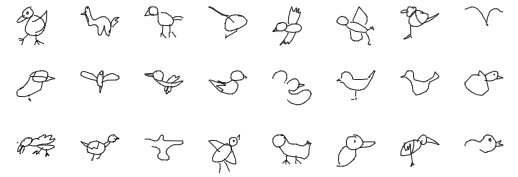
\includegraphics[width=0.55\textwidth]{img/quickdraw.png}
	\caption{Samples of QuickDraw dataset, by \cite{sketchrnn}}
	\label{fig:quickdraw}
\end{figure}
\begin{figure}[h]
	\centering
	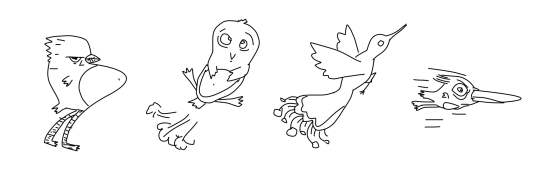
\includegraphics[width=0.45\textwidth]{img/doodlergan1.png}
	\caption{Samples from Creative Birds dataset by \cite{doodlergan}}
	\label{fig:doodlergan}
\end{figure}

Reinforcement learning was also applied to drawing generation, following the idea that drawing is a sequential decision-making process - see SPIRAL by \cite{ganin2018synthesizing} and SPIRAL++ \cite{mellor2019unsupervised}. These systems are expensive to train, as reinforcement agent receives feedback only in the end of drawing process, thus a lot of training attempts is required. 

Finally, in the work \cite{diffsvg} differentiable rasterizer was proposed and applied in different scenarios, including image generation with VAE and GAN. Wasserstein GAN was trained with a classification discriminator (real or fake), on MNIST dataset and cats from QuickDraw (see results on Figure \ref{fig:diffsvg}). In this project, we aim to train a generational model for more expressive Creative Birds dataset.

\subsection{Idea}
Generate artistic images using vector-graphic representation of strokes, differentiable rasterizer and GANs.

\paragraph{Hypothesis} We want to confirm that approach described in \cite{diffsvg} works for slightly more complex sketches - mainly we want to train WGAN for birds generation with differential rasterizer. See reported results from the paper on Figure \ref{fig:diffsvg} and samples from desired dataset on Figure \ref{fig:doodlergan}.

\paragraph{Future work} Inspired by ML-related artwork by Matty Mariansky, we may use differentiable renderer to create adversarial examples for object classification networks, or DeepDream-alike vector images. Also, strokes can be edited for additional coolness of resulting images. 

\section{Implementation details}
We start by reproducing the results from the original paper for a simple MNIST dataset, then moving to the new dataset.

\paragraph{Third-party code} We will use differentiable rendering from \cite{diffsvg} available at \href{https://github.com/BachiLi/diffvg}{github}. We will also use third-party datasets from QuickDraw used in \cite{sketchrnn} and DoodlerGAN from \cite{doodlergan} for experimenting.

\paragraph{Github} We will use a \href{https://github.com/ivanpuhachov/ift6756}{personal github repo}.

\paragraph{Resources} We will use one machine with NVidia 2080Ti GPU (11 GB) and Google Colab to run experiments in parallel.

\bibliography{example_paper}
\bibliographystyle{abbrvnat}

\begin{figure}[h]
	\centering
	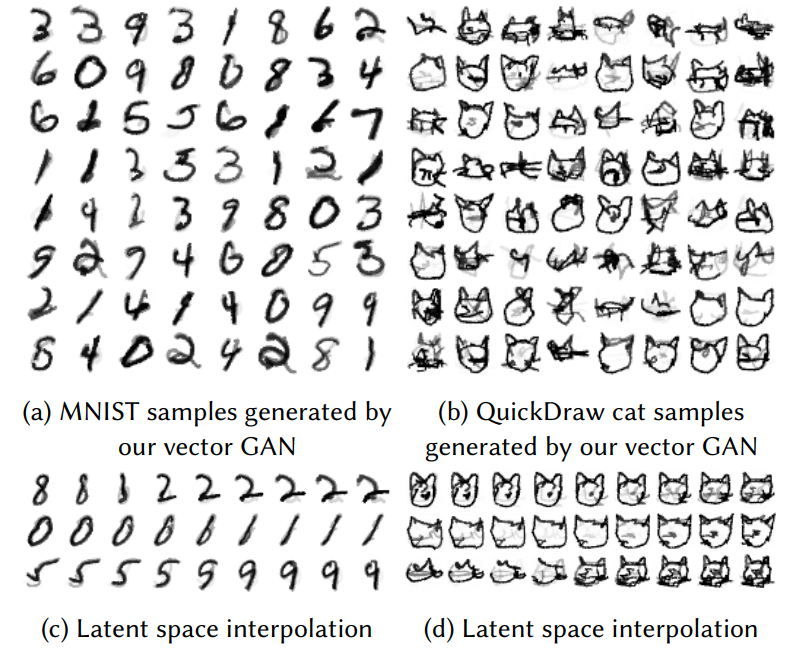
\includegraphics[width=0.65\textwidth]{img/diffsvg.png}
	\caption{Samples generated by GANs, screenshot directly from a paper by \cite{diffsvg}}
	\label{fig:diffsvg}
\end{figure}

\appendix 
\section{Additional figures}
\begin{figure}[h]
	\centering
	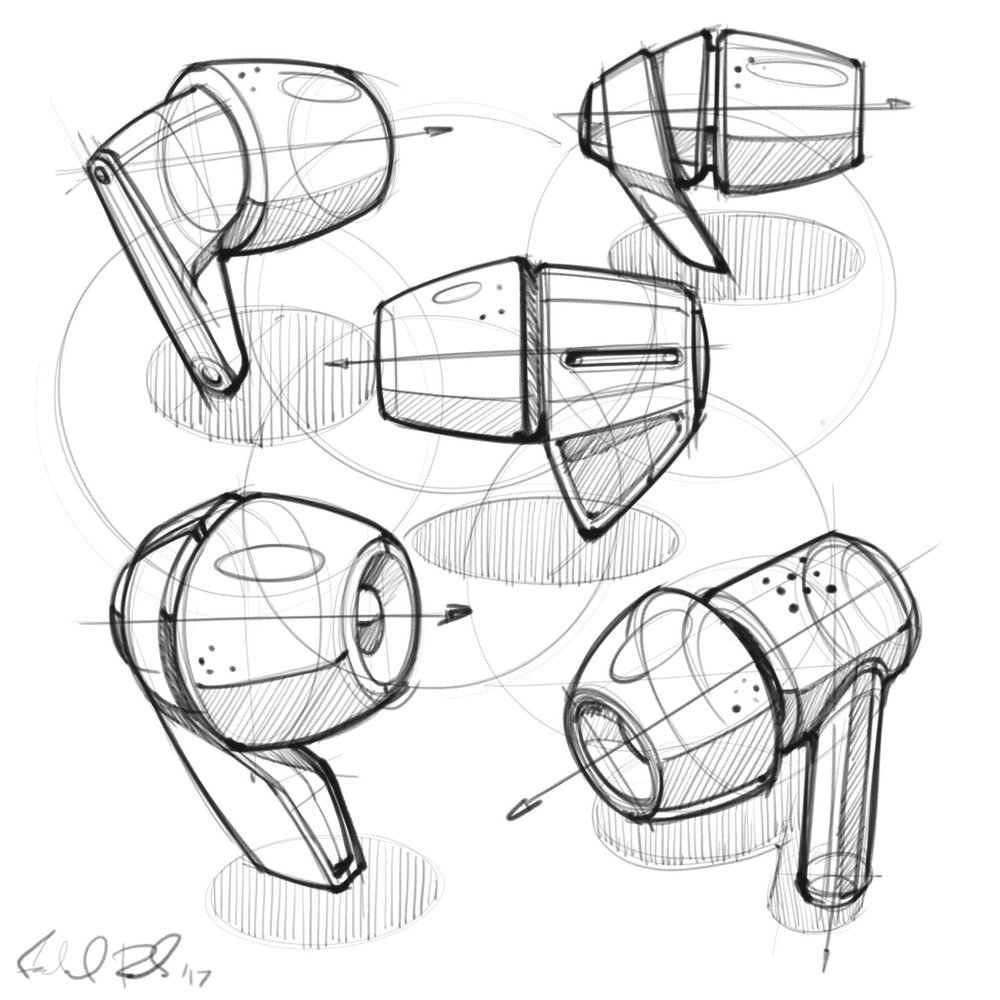
\includegraphics[width=0.35\textwidth]{img/sketch.jpeg}
	\caption{Example of a design sketch. Source: \href{https://fedriosdesign.com/design-sketching}{fedriodesign}}
	\label{fig:designsketch}
\end{figure}


\begin{figure}[h]
	\centering
	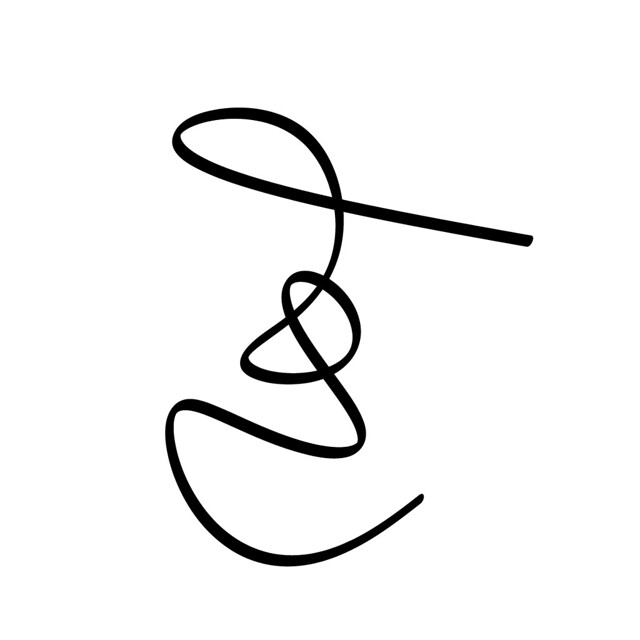
\includegraphics[width=0.55\textwidth]{img/face.jpg}
	\caption{"Evolutionary Faces (2020). A curve generator is pitted against a face recognition algorithm. Using an evolutionary process, the curves thrive to be more face-like. Limiting the curve to just a single or double line forces the generator to remain abstract". Description and image are taken from \href{http://www.aiartonline.com/highlights-2020/matty-mariansky/}{NeurIPS20 workshop}, art by Matty Mariansky}
	\label{fig:diffsvg}
\end{figure}

\end{document}